\documentclass[twoside]{book}

% Packages required by doxygen
\usepackage{fixltx2e}
\usepackage{calc}
\usepackage{doxygen}
\usepackage[export]{adjustbox} % also loads graphicx
\usepackage{graphicx}
\usepackage[utf8]{inputenc}
\usepackage{makeidx}
\usepackage{multicol}
\usepackage{multirow}
\PassOptionsToPackage{warn}{textcomp}
\usepackage{textcomp}
\usepackage[nointegrals]{wasysym}
\usepackage[table]{xcolor}

% Font selection
\usepackage[T1]{fontenc}
\usepackage[scaled=.90]{helvet}
\usepackage{courier}
\usepackage{amssymb}
\usepackage{sectsty}
\renewcommand{\familydefault}{\sfdefault}
\allsectionsfont{%
  \fontseries{bc}\selectfont%
  \color{darkgray}%
}
\renewcommand{\DoxyLabelFont}{%
  \fontseries{bc}\selectfont%
  \color{darkgray}%
}
\newcommand{\+}{\discretionary{\mbox{\scriptsize$\hookleftarrow$}}{}{}}

% Page & text layout
\usepackage{geometry}
\geometry{%
  a4paper,%
  top=2.5cm,%
  bottom=2.5cm,%
  left=2.5cm,%
  right=2.5cm%
}
\tolerance=750
\hfuzz=15pt
\hbadness=750
\setlength{\emergencystretch}{15pt}
\setlength{\parindent}{0cm}
\setlength{\parskip}{3ex plus 2ex minus 2ex}
\makeatletter
\renewcommand{\paragraph}{%
  \@startsection{paragraph}{4}{0ex}{-1.0ex}{1.0ex}{%
    \normalfont\normalsize\bfseries\SS@parafont%
  }%
}
\renewcommand{\subparagraph}{%
  \@startsection{subparagraph}{5}{0ex}{-1.0ex}{1.0ex}{%
    \normalfont\normalsize\bfseries\SS@subparafont%
  }%
}
\makeatother

% Headers & footers
\usepackage{fancyhdr}
\pagestyle{fancyplain}
\fancyhead[LE]{\fancyplain{}{\bfseries\thepage}}
\fancyhead[CE]{\fancyplain{}{}}
\fancyhead[RE]{\fancyplain{}{\bfseries\leftmark}}
\fancyhead[LO]{\fancyplain{}{\bfseries\rightmark}}
\fancyhead[CO]{\fancyplain{}{}}
\fancyhead[RO]{\fancyplain{}{\bfseries\thepage}}
\fancyfoot[LE]{\fancyplain{}{}}
\fancyfoot[CE]{\fancyplain{}{}}
\fancyfoot[RE]{\fancyplain{}{\bfseries\scriptsize Generated by Doxygen }}
\fancyfoot[LO]{\fancyplain{}{\bfseries\scriptsize Generated by Doxygen }}
\fancyfoot[CO]{\fancyplain{}{}}
\fancyfoot[RO]{\fancyplain{}{}}
\renewcommand{\footrulewidth}{0.4pt}
\renewcommand{\chaptermark}[1]{%
  \markboth{#1}{}%
}
\renewcommand{\sectionmark}[1]{%
  \markright{\thesection\ #1}%
}

% Indices & bibliography
\usepackage{natbib}
\usepackage[titles]{tocloft}
\setcounter{tocdepth}{3}
\setcounter{secnumdepth}{5}
\makeindex

% Hyperlinks (required, but should be loaded last)
\usepackage{ifpdf}
\ifpdf
  \usepackage[pdftex,pagebackref=true]{hyperref}
\else
  \usepackage[ps2pdf,pagebackref=true]{hyperref}
\fi
\hypersetup{%
  colorlinks=true,%
  linkcolor=blue,%
  citecolor=blue,%
  unicode%
}

% Custom commands
\newcommand{\clearemptydoublepage}{%
  \newpage{\pagestyle{empty}\cleardoublepage}%
}

\usepackage{caption}
\captionsetup{labelsep=space,justification=centering,font={bf},singlelinecheck=off,skip=4pt,position=top}

%===== C O N T E N T S =====

\begin{document}

% Titlepage & ToC
\hypersetup{pageanchor=false,
             bookmarksnumbered=true,
             pdfencoding=unicode
            }
\pagenumbering{alph}
\begin{titlepage}
\vspace*{7cm}
\begin{center}%
{\Large T\+I\+N\+Y\+S\+N74 \\[1ex]\large 0.\+6.\+0 }\\
\vspace*{1cm}
{\large Generated by Doxygen 1.8.13}\\
\end{center}
\end{titlepage}
\clearemptydoublepage
\pagenumbering{roman}
\tableofcontents
\clearemptydoublepage
\pagenumbering{arabic}
\hypersetup{pageanchor=true}

%--- Begin generated contents ---
\chapter{T\+I\+N\+Y\+S\+N74}
\label{index}\hypertarget{index}{}Library for Texas Instruments S\+N74\+H\+C595 Shift Registers (and clones), for use with A\+T\+T\+I\+NY chips.

Communication is currently bit-\/banging, with S\+PI in the works.

\subsection*{Usage}

Clone the repository into the \char`\"{}libraries\char`\"{} directory in your arduino installation directory.

The library includes two (2) header files\+:
\begin{DoxyItemize}
\item \hyperlink{tinysn74_8h}{tinysn74.\+h}
\item \hyperlink{tinysn74__config_8h}{tinysn74\+\_\+config.\+h}
\end{DoxyItemize}

The library provides several functions\+:
\begin{DoxyItemize}
\item sn\+Init -- This is called from within you sketch \hyperlink{SN74__Count_8ino_a4fc01d736fe50cf5b977f755b675f11d}{setup()} function
\item sn\+Shift (byte b$\ast$) -- This shifts the data out, requires an array to be passed in
\item sn\+Lat -- Latch shifted data to the output pins
\item sn\+Clr -- Clear the outputs
\item sn\+OE -- (Optional) Must be enabled in tinysn74\+\_\+config, allows triggering the output enable pin from within your program
\end{DoxyItemize}

\subsection*{Details}


\begin{DoxyItemize}
\item Current version\+: 0.\+6.\+0
\item Supports\+:
\begin{DoxyItemize}
\item A\+T\+Tinyx5 (25/45/85)
\item A\+T\+Tinyx4 (24/44/84) -\/ only minimally tested.
\end{DoxyItemize}
\end{DoxyItemize}

\subsection*{Pinouts}

\subsubsection*{S\+N74\+H\+C595}

Reference pinout of a S\+N75\+H\+C595 shift register.

Output H\textquotesingle{} is the \char`\"{}carry forward\char`\"{}. Use this to daisy-\/chain.

\tabulinesep=1mm
\begin{longtabu} spread 0pt [c]{*{5}{|X[-1]}|}
\hline
\rowcolor{\tableheadbgcolor}\textbf{ desc}&\textbf{ pin}&\textbf{ (P\+D\+I\+P/\+S\+O\+IC)}&\textbf{ pin}&\textbf{ desc  }\\\cline{1-5}
\endfirsthead
\hline
\endfoot
\hline
\rowcolor{\tableheadbgcolor}\textbf{ desc}&\textbf{ pin}&\textbf{ (P\+D\+I\+P/\+S\+O\+IC)}&\textbf{ pin}&\textbf{ desc  }\\\cline{1-5}
\endhead
Out B&1&---&16&V\+CC \\\cline{1-5}
Out C&2&---&15&Out A \\\cline{1-5}
Out D&3&---&14&Data In \\\cline{1-5}
Out E&4&---&13&OE \\\cline{1-5}
Out F&5&---&12&Latch \\\cline{1-5}
Out G&6&---&11&C\+LK \\\cline{1-5}
Out H&7&---&10&C\+LR \\\cline{1-5}
G\+ND&8&---&9&Out H\textquotesingle{} \\\cline{1-5}
\end{longtabu}
\subsubsection*{A\+T\+Tiny x5}

Default pinout for the A\+T\+Tiny 25/45/85 series. Note that M\+I\+SO is required if setting S\+PI Mode. Considering modifying the lib to also allow C\+LR to be an optional pin.

\tabulinesep=1mm
\begin{longtabu} spread 0pt [c]{*{5}{|X[-1]}|}
\hline
\rowcolor{\tableheadbgcolor}\textbf{ desc}&\textbf{ pin}&\textbf{ (P\+D\+I\+P/\+S\+O\+IC)}&\textbf{ pin}&\textbf{ desc  }\\\cline{1-5}
\endfirsthead
\hline
\endfoot
\hline
\rowcolor{\tableheadbgcolor}\textbf{ desc}&\textbf{ pin}&\textbf{ (P\+D\+I\+P/\+S\+O\+IC)}&\textbf{ pin}&\textbf{ desc  }\\\cline{1-5}
\endhead
R\+E\+S\+ET&1&---&8&V\+CC \\\cline{1-5}
C\+LR -\/ P\+B3&2&---&7&P\+B2 -\/ C\+LK \\\cline{1-5}
L\+AT -\/ P\+B4&3&---&6&P\+B1 -\/ M\+I\+SO \\\cline{1-5}
G\+ND&4&---&5&P\+B0 -\/ M\+O\+SI \\\cline{1-5}
\end{longtabu}


\subsubsection*{A\+T\+Tiny x4}

Default pinout for the A\+T\+Tiny 24/44/84 series. Note that M\+I\+SO is required if setting S\+PI Mode.

V0.\+0.\+1 Initial test pinout

Pins currently undefined in the library (i.\+e. available for use) are marked as \char`\"{}+++\char`\"{}

\tabulinesep=1mm
\begin{longtabu} spread 0pt [c]{*{5}{|X[-1]}|}
\hline
\rowcolor{\tableheadbgcolor}\textbf{ desc}&\textbf{ pin}&\textbf{ (P\+D\+I\+P/\+S\+O\+IC)}&\textbf{ pin}&\textbf{ desc  }\\\cline{1-5}
\endfirsthead
\hline
\endfoot
\hline
\rowcolor{\tableheadbgcolor}\textbf{ desc}&\textbf{ pin}&\textbf{ (P\+D\+I\+P/\+S\+O\+IC)}&\textbf{ pin}&\textbf{ desc  }\\\cline{1-5}
\endhead
V\+CC&1&---&14&G\+ND \\\cline{1-5}
+++ P\+B0&2&---&13&P\+A0 +++ \\\cline{1-5}
+++ P\+B1&3&---&12&P\+A1 +++ \\\cline{1-5}
R\+E\+S\+ET&4&---&11&P\+A2 +++ \\\cline{1-5}
+++ P\+B2&5&---&10&P\+A3 -\/ C\+LR \\\cline{1-5}
L\+AT -\/ P\+A7&6&---&9&P\+A4 -\/ C\+LK \\\cline{1-5}
M\+O\+SI -\/ P\+A6&7&---&8&P\+A5 -\/ M\+I\+SO \\\cline{1-5}
\end{longtabu}
\subsection*{Attribution}

Lots of influence from lots of places, mainly the sparkfun repo for the T\+L\+C5940 driver. Thanks to one and all for sharing your solutions.

\subsection*{Changelog}

0.\+6.\+0 -\/ Added example sketch, fixed math errors causing the library to eat significantly more R\+AM than necessary. 
\chapter{File Index}
\section{File List}
Here is a list of all documented files with brief descriptions\+:\begin{DoxyCompactList}
\item\contentsline{section}{examples/\+S\+N74\+\_\+\+Count/\hyperlink{SN74__Count_8ino}{S\+N74\+\_\+\+Count.\+ino} \\*This short example counts from 0 to 255 }{\pageref{SN74__Count_8ino}}{}
\item\contentsline{section}{examples/\+S\+N74\+\_\+\+Random\+Blink/\hyperlink{SN74__RandomBlink_8ino}{S\+N74\+\_\+\+Random\+Blink.\+ino} \\*A more involved example }{\pageref{SN74__RandomBlink_8ino}}{}
\item\contentsline{section}{src/\hyperlink{tinysn74_8c}{tinysn74.\+c} \\*Library to drive S\+N74\+H\+C595 chips with A\+T\+Tiny microcontrollers }{\pageref{tinysn74_8c}}{}
\item\contentsline{section}{src/\hyperlink{tinysn74_8h}{tinysn74.\+h} }{\pageref{tinysn74_8h}}{}
\item\contentsline{section}{src/\hyperlink{tinysn74__config_8h}{tinysn74\+\_\+config.\+h} \\*Master configuration file for the tinysn74 library }{\pageref{tinysn74__config_8h}}{}
\item\contentsline{section}{src/pinouts/{\bfseries A\+Ttinyx4.\+h} }{\pageref{ATtinyx4_8h}}{}
\item\contentsline{section}{src/pinouts/{\bfseries A\+Ttinyx5.\+h} }{\pageref{ATtinyx5_8h}}{}
\item\contentsline{section}{src/pinouts/{\bfseries chips.\+h} }{\pageref{chips_8h}}{}
\end{DoxyCompactList}

\chapter{File Documentation}
\hypertarget{SN74__Count_8ino}{}\section{examples/\+S\+N74\+\_\+\+Count/\+S\+N74\+\_\+\+Count.ino File Reference}
\label{SN74__Count_8ino}\index{examples/\+S\+N74\+\_\+\+Count/\+S\+N74\+\_\+\+Count.\+ino@{examples/\+S\+N74\+\_\+\+Count/\+S\+N74\+\_\+\+Count.\+ino}}


This short example counts from 0 to 255.  


{\ttfamily \#include $<$tinysn74.\+h$>$}\newline
Include dependency graph for S\+N74\+\_\+\+Count.\+ino\+:\nopagebreak
\begin{figure}[H]
\begin{center}
\leavevmode
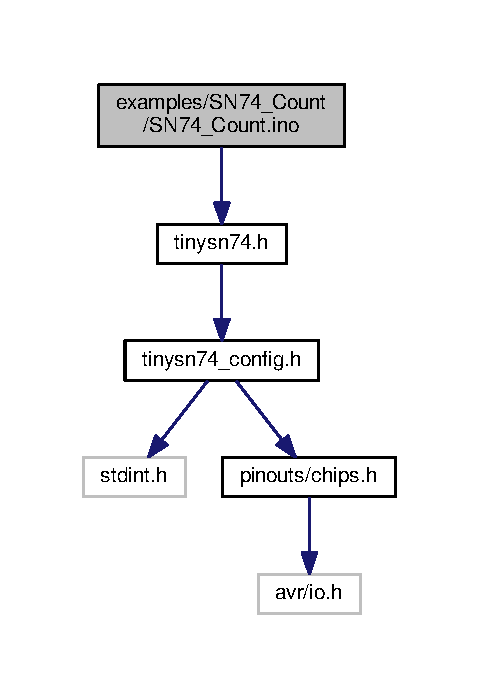
\includegraphics[width=230pt]{SN74__Count_8ino__incl}
\end{center}
\end{figure}
\subsection*{Functions}
\begin{DoxyCompactItemize}
\item 
void \hyperlink{SN74__Count_8ino_a4fc01d736fe50cf5b977f755b675f11d}{setup} ()
\begin{DoxyCompactList}\small\item\em Initial setup code. Runs once at power-\/on or chip reset. \end{DoxyCompactList}\item 
void \hyperlink{SN74__Count_8ino_afe461d27b9c48d5921c00d521181f12f}{loop} ()
\begin{DoxyCompactList}\small\item\em Main program loop. \end{DoxyCompactList}\end{DoxyCompactItemize}
\subsection*{Variables}
\begin{DoxyCompactItemize}
\item 
uint8\+\_\+t \hyperlink{SN74__Count_8ino_af27e3188294c2df66d975b74a09c001d}{i} =0
\begin{DoxyCompactList}\small\item\em Counter. \end{DoxyCompactList}\item 
uint8\+\_\+t \hyperlink{SN74__Count_8ino_a089fa212b87b3656b0a264a5e4457d8e}{chip} \mbox{[}1\mbox{]}
\begin{DoxyCompactList}\small\item\em Create the chip array. \end{DoxyCompactList}\end{DoxyCompactItemize}


\subsection{Detailed Description}
This short example counts from 0 to 255. 

This simple sketch is intended to help verify the S\+N74 is properly connected to the microcontroller 

\subsection{Function Documentation}
\mbox{\Hypertarget{SN74__Count_8ino_afe461d27b9c48d5921c00d521181f12f}\label{SN74__Count_8ino_afe461d27b9c48d5921c00d521181f12f}} 
\index{S\+N74\+\_\+\+Count.\+ino@{S\+N74\+\_\+\+Count.\+ino}!loop@{loop}}
\index{loop@{loop}!S\+N74\+\_\+\+Count.\+ino@{S\+N74\+\_\+\+Count.\+ino}}
\subsubsection{\texorpdfstring{loop()}{loop()}}
{\footnotesize\ttfamily void loop (\begin{DoxyParamCaption}{ }\end{DoxyParamCaption})}



Main program loop. 

Runs indefinitely. \mbox{\Hypertarget{SN74__Count_8ino_a4fc01d736fe50cf5b977f755b675f11d}\label{SN74__Count_8ino_a4fc01d736fe50cf5b977f755b675f11d}} 
\index{S\+N74\+\_\+\+Count.\+ino@{S\+N74\+\_\+\+Count.\+ino}!setup@{setup}}
\index{setup@{setup}!S\+N74\+\_\+\+Count.\+ino@{S\+N74\+\_\+\+Count.\+ino}}
\subsubsection{\texorpdfstring{setup()}{setup()}}
{\footnotesize\ttfamily void setup (\begin{DoxyParamCaption}{ }\end{DoxyParamCaption})}



Initial setup code. Runs once at power-\/on or chip reset. 



\subsection{Variable Documentation}
\mbox{\Hypertarget{SN74__Count_8ino_a089fa212b87b3656b0a264a5e4457d8e}\label{SN74__Count_8ino_a089fa212b87b3656b0a264a5e4457d8e}} 
\index{S\+N74\+\_\+\+Count.\+ino@{S\+N74\+\_\+\+Count.\+ino}!chip@{chip}}
\index{chip@{chip}!S\+N74\+\_\+\+Count.\+ino@{S\+N74\+\_\+\+Count.\+ino}}
\subsubsection{\texorpdfstring{chip}{chip}}
{\footnotesize\ttfamily uint8\+\_\+t chip\mbox{[}1\mbox{]}}



Create the chip array. 

\mbox{\Hypertarget{SN74__Count_8ino_af27e3188294c2df66d975b74a09c001d}\label{SN74__Count_8ino_af27e3188294c2df66d975b74a09c001d}} 
\index{S\+N74\+\_\+\+Count.\+ino@{S\+N74\+\_\+\+Count.\+ino}!i@{i}}
\index{i@{i}!S\+N74\+\_\+\+Count.\+ino@{S\+N74\+\_\+\+Count.\+ino}}
\subsubsection{\texorpdfstring{i}{i}}
{\footnotesize\ttfamily uint8\+\_\+t i =0}



Counter. 


\hypertarget{SN74__RandomBlink_8ino}{}\section{examples/\+S\+N74\+\_\+\+Random\+Blink/\+S\+N74\+\_\+\+Random\+Blink.ino File Reference}
\label{SN74__RandomBlink_8ino}\index{examples/\+S\+N74\+\_\+\+Random\+Blink/\+S\+N74\+\_\+\+Random\+Blink.\+ino@{examples/\+S\+N74\+\_\+\+Random\+Blink/\+S\+N74\+\_\+\+Random\+Blink.\+ino}}


A more involved example.  


{\ttfamily \#include $<$tinysn74.\+h$>$}\newline
Include dependency graph for S\+N74\+\_\+\+Random\+Blink.\+ino\+:\nopagebreak
\begin{figure}[H]
\begin{center}
\leavevmode
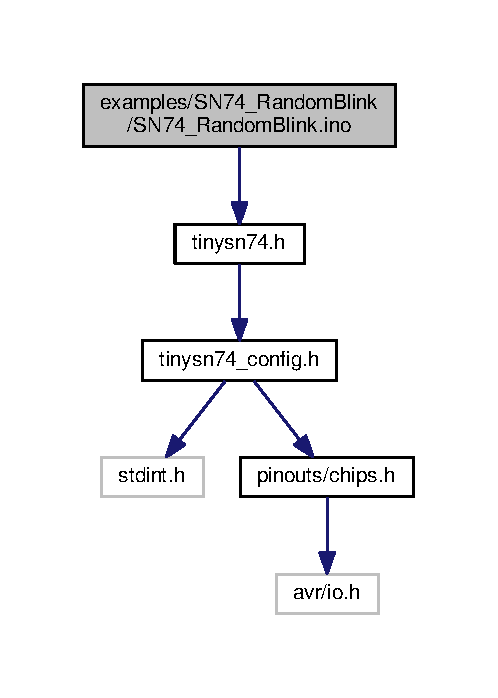
\includegraphics[width=239pt]{SN74__RandomBlink_8ino__incl}
\end{center}
\end{figure}
\subsection*{Functions}
\begin{DoxyCompactItemize}
\item 
void \hyperlink{SN74__RandomBlink_8ino_a4fc01d736fe50cf5b977f755b675f11d}{setup} ()
\begin{DoxyCompactList}\small\item\em Program initialization. \end{DoxyCompactList}\item 
void \hyperlink{SN74__RandomBlink_8ino_a9069fa50959f53362dad0f5038f45d60}{randlite} ()
\begin{DoxyCompactList}\small\item\em Randomly select the chip and pin to change state. \end{DoxyCompactList}\item 
void \hyperlink{SN74__RandomBlink_8ino_afe461d27b9c48d5921c00d521181f12f}{loop} ()
\begin{DoxyCompactList}\small\item\em Main program loop. \end{DoxyCompactList}\end{DoxyCompactItemize}
\subsection*{Variables}
\begin{DoxyCompactItemize}
\item 
uint8\+\_\+t \hyperlink{SN74__RandomBlink_8ino_aab45faad5b835d77a869fca4747ab75d}{chp} = 0
\begin{DoxyCompactList}\small\item\em Chip select value. \end{DoxyCompactList}\item 
uint8\+\_\+t \hyperlink{SN74__RandomBlink_8ino_ad1a4ecf3125fbcc9447f70f7361f2fb0}{rnd} = 0
\begin{DoxyCompactList}\small\item\em R\+NG value. \end{DoxyCompactList}\item 
uint8\+\_\+t \hyperlink{SN74__RandomBlink_8ino_a4bc5cfe94d996891a734c6c645f44e45}{chip} \mbox{[}N\+U\+M\+S\+N74\mbox{]}
\begin{DoxyCompactList}\small\item\em Chip array. \end{DoxyCompactList}\item 
uint8\+\_\+t \hyperlink{SN74__RandomBlink_8ino_a74fac0365dddec359ec40da99dde9d8a}{pina} \mbox{[}8\mbox{]} =\{0x01,0x02,0x04,0x08,0x10,0x20,0x40,0x80\}
\begin{DoxyCompactList}\small\item\em Integer to pin conversion. \end{DoxyCompactList}\item 
uint8\+\_\+t \hyperlink{SN74__RandomBlink_8ino_a6dc166123fed68e9b34a2512623163e0}{on} = 1
\begin{DoxyCompactList}\small\item\em Indicator for enabling outputs. \end{DoxyCompactList}\item 
int \hyperlink{SN74__RandomBlink_8ino_aaefdb10b18059f3c08332338630b3f68}{wait} =0
\begin{DoxyCompactList}\small\item\em Indicate loop should delay. \end{DoxyCompactList}\item 
uint8\+\_\+t \hyperlink{SN74__RandomBlink_8ino_af27e3188294c2df66d975b74a09c001d}{i} =0
\begin{DoxyCompactList}\small\item\em Counter for walking the chip array. \end{DoxyCompactList}\end{DoxyCompactItemize}


\subsection{Detailed Description}
A more involved example. 

This example sketch shows how this library can be utilized to create complex effects. In this case, we\textquotesingle{}re selecting a random pin on a random chip to light. 

\subsection{Function Documentation}
\mbox{\Hypertarget{SN74__RandomBlink_8ino_afe461d27b9c48d5921c00d521181f12f}\label{SN74__RandomBlink_8ino_afe461d27b9c48d5921c00d521181f12f}} 
\index{S\+N74\+\_\+\+Random\+Blink.\+ino@{S\+N74\+\_\+\+Random\+Blink.\+ino}!loop@{loop}}
\index{loop@{loop}!S\+N74\+\_\+\+Random\+Blink.\+ino@{S\+N74\+\_\+\+Random\+Blink.\+ino}}
\subsubsection{\texorpdfstring{loop()}{loop()}}
{\footnotesize\ttfamily void loop (\begin{DoxyParamCaption}{ }\end{DoxyParamCaption})}



Main program loop. 

Infinite loop to continually call \hyperlink{SN74__RandomBlink_8ino_a9069fa50959f53362dad0f5038f45d60}{randlite()}, and wait 100 ms after every execution. \mbox{\Hypertarget{SN74__RandomBlink_8ino_a9069fa50959f53362dad0f5038f45d60}\label{SN74__RandomBlink_8ino_a9069fa50959f53362dad0f5038f45d60}} 
\index{S\+N74\+\_\+\+Random\+Blink.\+ino@{S\+N74\+\_\+\+Random\+Blink.\+ino}!randlite@{randlite}}
\index{randlite@{randlite}!S\+N74\+\_\+\+Random\+Blink.\+ino@{S\+N74\+\_\+\+Random\+Blink.\+ino}}
\subsubsection{\texorpdfstring{randlite()}{randlite()}}
{\footnotesize\ttfamily void randlite (\begin{DoxyParamCaption}{ }\end{DoxyParamCaption})}



Randomly select the chip and pin to change state. 

Provided that N\+U\+M\+S\+N74 $>$1, this will randomly select a pin and chip from their respective arrays, and set the output state accordingly. Once the data is shifted out and latched in, the function determines if the whole array\textquotesingle{}s outputs are logic high or logic low, in order to determine if the other cycle should be started. \mbox{\Hypertarget{SN74__RandomBlink_8ino_a4fc01d736fe50cf5b977f755b675f11d}\label{SN74__RandomBlink_8ino_a4fc01d736fe50cf5b977f755b675f11d}} 
\index{S\+N74\+\_\+\+Random\+Blink.\+ino@{S\+N74\+\_\+\+Random\+Blink.\+ino}!setup@{setup}}
\index{setup@{setup}!S\+N74\+\_\+\+Random\+Blink.\+ino@{S\+N74\+\_\+\+Random\+Blink.\+ino}}
\subsubsection{\texorpdfstring{setup()}{setup()}}
{\footnotesize\ttfamily void setup (\begin{DoxyParamCaption}{ }\end{DoxyParamCaption})}



Program initialization. 

Runs once at power on or microcontroller reset. Calls \hyperlink{tinysn74_8c_a75d55e672f3f4dd06cd0c73479f64ade}{sn\+Init()} and seeds the P\+R\+NG with the number of microseconds since the chip (re) booted. 

\subsection{Variable Documentation}
\mbox{\Hypertarget{SN74__RandomBlink_8ino_a4bc5cfe94d996891a734c6c645f44e45}\label{SN74__RandomBlink_8ino_a4bc5cfe94d996891a734c6c645f44e45}} 
\index{S\+N74\+\_\+\+Random\+Blink.\+ino@{S\+N74\+\_\+\+Random\+Blink.\+ino}!chip@{chip}}
\index{chip@{chip}!S\+N74\+\_\+\+Random\+Blink.\+ino@{S\+N74\+\_\+\+Random\+Blink.\+ino}}
\subsubsection{\texorpdfstring{chip}{chip}}
{\footnotesize\ttfamily uint8\+\_\+t chip\mbox{[}N\+U\+M\+S\+N74\mbox{]}}



Chip array. 

8-\/bit unsigned integer array holds the values for the pin(s) that are active on any one chip.

Array is in \char`\"{}most significant chip first\char`\"{} order -- that is, chip\mbox{[}0\mbox{]} is the S\+N74\+H\+C595 chip that is farthest away. chip\mbox{[}N\+U\+M\+S\+N74-\/1\mbox{]} is the chip directly connected to M\+O\+SI \mbox{\Hypertarget{SN74__RandomBlink_8ino_aab45faad5b835d77a869fca4747ab75d}\label{SN74__RandomBlink_8ino_aab45faad5b835d77a869fca4747ab75d}} 
\index{S\+N74\+\_\+\+Random\+Blink.\+ino@{S\+N74\+\_\+\+Random\+Blink.\+ino}!chp@{chp}}
\index{chp@{chp}!S\+N74\+\_\+\+Random\+Blink.\+ino@{S\+N74\+\_\+\+Random\+Blink.\+ino}}
\subsubsection{\texorpdfstring{chp}{chp}}
{\footnotesize\ttfamily uint8\+\_\+t chp = 0}



Chip select value. 

uint8\+\_\+t as 255 is more than a Tiny2x or 4x chip can run; so this saves a bit of R\+AM. Change to uint16\+\_\+t if you\textquotesingle{}re using a Tiny8x and want to run more than 255 S\+N74\+H\+C595 \mbox{\Hypertarget{SN74__RandomBlink_8ino_af27e3188294c2df66d975b74a09c001d}\label{SN74__RandomBlink_8ino_af27e3188294c2df66d975b74a09c001d}} 
\index{S\+N74\+\_\+\+Random\+Blink.\+ino@{S\+N74\+\_\+\+Random\+Blink.\+ino}!i@{i}}
\index{i@{i}!S\+N74\+\_\+\+Random\+Blink.\+ino@{S\+N74\+\_\+\+Random\+Blink.\+ino}}
\subsubsection{\texorpdfstring{i}{i}}
{\footnotesize\ttfamily uint8\+\_\+t i =0}



Counter for walking the chip array. 

Set to uint8\+\_\+t, as Tiny2x/4x will never exceed 255 S\+N74 chips; so this saves some R\+AM. Change to uint16\+\_\+t for a tiny8x if you choose to use more than 255 chips. \mbox{\Hypertarget{SN74__RandomBlink_8ino_a6dc166123fed68e9b34a2512623163e0}\label{SN74__RandomBlink_8ino_a6dc166123fed68e9b34a2512623163e0}} 
\index{S\+N74\+\_\+\+Random\+Blink.\+ino@{S\+N74\+\_\+\+Random\+Blink.\+ino}!on@{on}}
\index{on@{on}!S\+N74\+\_\+\+Random\+Blink.\+ino@{S\+N74\+\_\+\+Random\+Blink.\+ino}}
\subsubsection{\texorpdfstring{on}{on}}
{\footnotesize\ttfamily uint8\+\_\+t on = 1}



Indicator for enabling outputs. 

When 1, the output selected in this run will be set logic high. When 0, output will be set to logic low. \mbox{\Hypertarget{SN74__RandomBlink_8ino_a74fac0365dddec359ec40da99dde9d8a}\label{SN74__RandomBlink_8ino_a74fac0365dddec359ec40da99dde9d8a}} 
\index{S\+N74\+\_\+\+Random\+Blink.\+ino@{S\+N74\+\_\+\+Random\+Blink.\+ino}!pina@{pina}}
\index{pina@{pina}!S\+N74\+\_\+\+Random\+Blink.\+ino@{S\+N74\+\_\+\+Random\+Blink.\+ino}}
\subsubsection{\texorpdfstring{pina}{pina}}
{\footnotesize\ttfamily uint8\+\_\+t pina\mbox{[}8\mbox{]} =\{0x01,0x02,0x04,0x08,0x10,0x20,0x40,0x80\}}



Integer to pin conversion. 

If we just used a value 0-\/255, we\textquotesingle{}d get however many pins lit, corresponding to the decimal -\/$>$ binary conversion of a random number. That is, if we fed chip\mbox{[}n\mbox{]} a value of 133, pins 8, 3, and 1 would light (corresponding to 128 + 4 + 1), and that\textquotesingle{}s not what we want.

Array\+Value = Hex (decimal)
\begin{DoxyItemize}
\item \mbox{[}0\mbox{]} = 0x01 (1)
\item \mbox{[}1\mbox{]} = 0x02 (2)
\item \mbox{[}2\mbox{]} = 0x04 (4)
\item \mbox{[}3\mbox{]} = 0x08 (8)
\item \mbox{[}4\mbox{]} = 0x10 (16)
\item \mbox{[}5\mbox{]} = 0x20 (32)
\item \mbox{[}6\mbox{]} = 0x40 (64)
\item \mbox{[}7\mbox{]} = 0x80 (128) 
\end{DoxyItemize}\mbox{\Hypertarget{SN74__RandomBlink_8ino_ad1a4ecf3125fbcc9447f70f7361f2fb0}\label{SN74__RandomBlink_8ino_ad1a4ecf3125fbcc9447f70f7361f2fb0}} 
\index{S\+N74\+\_\+\+Random\+Blink.\+ino@{S\+N74\+\_\+\+Random\+Blink.\+ino}!rnd@{rnd}}
\index{rnd@{rnd}!S\+N74\+\_\+\+Random\+Blink.\+ino@{S\+N74\+\_\+\+Random\+Blink.\+ino}}
\subsubsection{\texorpdfstring{rnd}{rnd}}
{\footnotesize\ttfamily uint8\+\_\+t rnd = 0}



R\+NG value. 

Value for the pin we\textquotesingle{}re going to light \mbox{\Hypertarget{SN74__RandomBlink_8ino_aaefdb10b18059f3c08332338630b3f68}\label{SN74__RandomBlink_8ino_aaefdb10b18059f3c08332338630b3f68}} 
\index{S\+N74\+\_\+\+Random\+Blink.\+ino@{S\+N74\+\_\+\+Random\+Blink.\+ino}!wait@{wait}}
\index{wait@{wait}!S\+N74\+\_\+\+Random\+Blink.\+ino@{S\+N74\+\_\+\+Random\+Blink.\+ino}}
\subsubsection{\texorpdfstring{wait}{wait}}
{\footnotesize\ttfamily int wait =0}



Indicate loop should delay. 

When 1, loop will delay for N seconds (default 5) before switching state. That is, if all the outputs just finished going logic high, wait before setting random outputs to logic low (or vice-\/versa). 
\hypertarget{tinysn74_8c}{}\section{src/tinysn74.c File Reference}
\label{tinysn74_8c}\index{src/tinysn74.\+c@{src/tinysn74.\+c}}


Library to drive S\+N74\+H\+C595 chips with A\+T\+Tiny microcontrollers.  


{\ttfamily \#include $<$avr/interrupt.\+h$>$}\newline
{\ttfamily \#include $<$util/delay.\+h$>$}\newline
{\ttfamily \#include \char`\"{}tinysn74\+\_\+config.\+h\char`\"{}}\newline
{\ttfamily \#include \char`\"{}tinysn74.\+h\char`\"{}}\newline
Include dependency graph for tinysn74.\+c\+:\nopagebreak
\begin{figure}[H]
\begin{center}
\leavevmode
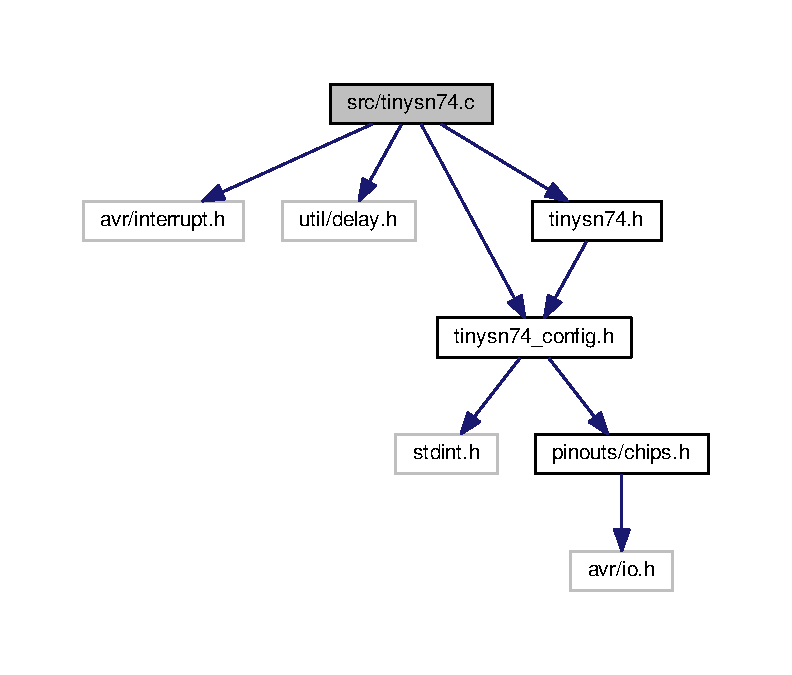
\includegraphics[width=350pt]{tinysn74_8c__incl}
\end{center}
\end{figure}
\subsection*{Macros}
\begin{DoxyCompactItemize}
\item 
\#define \hyperlink{tinysn74_8c_ad72dbcf6d0153db1b8d8a58001feed83}{D\+E\+B\+UG}~1
\begin{DoxyCompactList}\small\item\em A\+VR Interrupt Library. \end{DoxyCompactList}\item 
\#define \hyperlink{tinysn74_8c_a4330aeed1c9cef86f25a77fc7d5c28e6}{pulse}(port,  pin)~port $\vert$= \+\_\+\+BV(pin); port \&= $\sim$\+\_\+\+BV(pin);
\begin{DoxyCompactList}\small\item\em sends a pulse to the pin (i.\+e. set logic high, then low) \end{DoxyCompactList}\item 
\#define \hyperlink{tinysn74_8c_aa8f7441d0691c9e378f74be062aa73e1}{hi}(port,  pin)~port $\vert$= \+\_\+\+BV(pin);
\begin{DoxyCompactList}\small\item\em pulls a pin logic high \end{DoxyCompactList}\item 
\#define \hyperlink{tinysn74_8c_a2bd7cc1ea865db8275b9528b3dbb5793}{lo}(port,  pin)~port \&= $\sim$\+\_\+\+BV(pin);
\begin{DoxyCompactList}\small\item\em pulls a pin logic low \end{DoxyCompactList}\end{DoxyCompactItemize}
\subsection*{Functions}
\begin{DoxyCompactItemize}
\item 
void \hyperlink{tinysn74_8c_a75d55e672f3f4dd06cd0c73479f64ade}{sn\+Init} (void)
\begin{DoxyCompactList}\small\item\em Initializes the library. \end{DoxyCompactList}\item 
void \hyperlink{tinysn74_8c_ad06bf9aab33483c64594a58e072279fe}{sn\+C\+LR} (void)
\begin{DoxyCompactList}\small\item\em Clear the output register. \end{DoxyCompactList}\item 
void \hyperlink{tinysn74_8c_ace8f256b6c1b7e959f1d486b8796cb58}{sn\+OE} (uint8\+\_\+t off)
\begin{DoxyCompactList}\small\item\em Enable / disable S\+N74 outputs. \end{DoxyCompactList}\item 
void \hyperlink{tinysn74_8c_ac9f372294bcbd3d976f30953e2aaeb1b}{sn\+Shift\+Init} (void)
\begin{DoxyCompactList}\small\item\em Initializes the shifting logic. \end{DoxyCompactList}\item 
void \hyperlink{tinysn74_8c_aedfd23cb2c8f35f1fd274ad3d9395ad8}{sn\+Shift} (uint8\+\_\+t $\ast$b)
\begin{DoxyCompactList}\small\item\em Shifting logic to get data from the micro to the shift registers. \end{DoxyCompactList}\item 
void \hyperlink{tinysn74_8c_ae57a50787422eaee268c496d51f8dc00}{sn\+Lat} (void)
\begin{DoxyCompactList}\small\item\em Latcn data from S\+N74\textquotesingle{}s internal shift register to the output. \end{DoxyCompactList}\end{DoxyCompactItemize}


\subsection{Detailed Description}
Library to drive S\+N74\+H\+C595 chips with A\+T\+Tiny microcontrollers. 

This library provides the necessary hooks for you to control Texas Instruments S\+N74\+H\+C595 shift registers (or equivalent). 

\subsection{Macro Definition Documentation}
\mbox{\Hypertarget{tinysn74_8c_ad72dbcf6d0153db1b8d8a58001feed83}\label{tinysn74_8c_ad72dbcf6d0153db1b8d8a58001feed83}} 
\index{tinysn74.\+c@{tinysn74.\+c}!D\+E\+B\+UG@{D\+E\+B\+UG}}
\index{D\+E\+B\+UG@{D\+E\+B\+UG}!tinysn74.\+c@{tinysn74.\+c}}
\subsubsection{\texorpdfstring{D\+E\+B\+UG}{DEBUG}}
{\footnotesize\ttfamily \#define D\+E\+B\+UG~1}



A\+VR Interrupt Library. 

A\+VR IO Library\+For \+\_\+delay\+\_\+ms() Library configuration file Library headers D\+E\+B\+UG = 1 for debugging / slowing things down \mbox{\Hypertarget{tinysn74_8c_aa8f7441d0691c9e378f74be062aa73e1}\label{tinysn74_8c_aa8f7441d0691c9e378f74be062aa73e1}} 
\index{tinysn74.\+c@{tinysn74.\+c}!hi@{hi}}
\index{hi@{hi}!tinysn74.\+c@{tinysn74.\+c}}
\subsubsection{\texorpdfstring{hi}{hi}}
{\footnotesize\ttfamily \#define hi(\begin{DoxyParamCaption}\item[{}]{port,  }\item[{}]{pin }\end{DoxyParamCaption})~port $\vert$= \+\_\+\+BV(pin);}



pulls a pin logic high 

\mbox{\Hypertarget{tinysn74_8c_a2bd7cc1ea865db8275b9528b3dbb5793}\label{tinysn74_8c_a2bd7cc1ea865db8275b9528b3dbb5793}} 
\index{tinysn74.\+c@{tinysn74.\+c}!lo@{lo}}
\index{lo@{lo}!tinysn74.\+c@{tinysn74.\+c}}
\subsubsection{\texorpdfstring{lo}{lo}}
{\footnotesize\ttfamily \#define lo(\begin{DoxyParamCaption}\item[{}]{port,  }\item[{}]{pin }\end{DoxyParamCaption})~port \&= $\sim$\+\_\+\+BV(pin);}



pulls a pin logic low 

\mbox{\Hypertarget{tinysn74_8c_a4330aeed1c9cef86f25a77fc7d5c28e6}\label{tinysn74_8c_a4330aeed1c9cef86f25a77fc7d5c28e6}} 
\index{tinysn74.\+c@{tinysn74.\+c}!pulse@{pulse}}
\index{pulse@{pulse}!tinysn74.\+c@{tinysn74.\+c}}
\subsubsection{\texorpdfstring{pulse}{pulse}}
{\footnotesize\ttfamily \#define pulse(\begin{DoxyParamCaption}\item[{}]{port,  }\item[{}]{pin }\end{DoxyParamCaption})~port $\vert$= \+\_\+\+BV(pin); port \&= $\sim$\+\_\+\+BV(pin);}



sends a pulse to the pin (i.\+e. set logic high, then low) 



\subsection{Function Documentation}
\mbox{\Hypertarget{tinysn74_8c_ad06bf9aab33483c64594a58e072279fe}\label{tinysn74_8c_ad06bf9aab33483c64594a58e072279fe}} 
\index{tinysn74.\+c@{tinysn74.\+c}!sn\+C\+LR@{sn\+C\+LR}}
\index{sn\+C\+LR@{sn\+C\+LR}!tinysn74.\+c@{tinysn74.\+c}}
\subsubsection{\texorpdfstring{sn\+C\+L\+R()}{snCLR()}}
{\footnotesize\ttfamily void sn\+C\+LR (\begin{DoxyParamCaption}\item[{void}]{ }\end{DoxyParamCaption})}



Clear the output register. 

This function will clear all outputs of the connected S\+N74 chips, without having to shift in N bytes of 0x00 \mbox{\Hypertarget{tinysn74_8c_a75d55e672f3f4dd06cd0c73479f64ade}\label{tinysn74_8c_a75d55e672f3f4dd06cd0c73479f64ade}} 
\index{tinysn74.\+c@{tinysn74.\+c}!sn\+Init@{sn\+Init}}
\index{sn\+Init@{sn\+Init}!tinysn74.\+c@{tinysn74.\+c}}
\subsubsection{\texorpdfstring{sn\+Init()}{snInit()}}
{\footnotesize\ttfamily void sn\+Init (\begin{DoxyParamCaption}\item[{void}]{ }\end{DoxyParamCaption})}



Initializes the library. 

This function sets up the ports / pins of the A\+T\+T\+I\+NY to output, and clears the output registers of the connected shift register(s). \mbox{\Hypertarget{tinysn74_8c_ae57a50787422eaee268c496d51f8dc00}\label{tinysn74_8c_ae57a50787422eaee268c496d51f8dc00}} 
\index{tinysn74.\+c@{tinysn74.\+c}!sn\+Lat@{sn\+Lat}}
\index{sn\+Lat@{sn\+Lat}!tinysn74.\+c@{tinysn74.\+c}}
\subsubsection{\texorpdfstring{sn\+Lat()}{snLat()}}
{\footnotesize\ttfamily void sn\+Lat (\begin{DoxyParamCaption}\item[{void}]{ }\end{DoxyParamCaption})}



Latcn data from S\+N74\textquotesingle{}s internal shift register to the output. 

This function is what actually sets the output pins to the value contained in the input shift register. Without calling this, the pins will never go logic high (or logic low). \mbox{\Hypertarget{tinysn74_8c_ace8f256b6c1b7e959f1d486b8796cb58}\label{tinysn74_8c_ace8f256b6c1b7e959f1d486b8796cb58}} 
\index{tinysn74.\+c@{tinysn74.\+c}!sn\+OE@{sn\+OE}}
\index{sn\+OE@{sn\+OE}!tinysn74.\+c@{tinysn74.\+c}}
\subsubsection{\texorpdfstring{sn\+O\+E()}{snOE()}}
{\footnotesize\ttfamily void sn\+OE (\begin{DoxyParamCaption}\item[{uint8\+\_\+t}]{off }\end{DoxyParamCaption})}



Enable / disable S\+N74 outputs. 

If the sn\+OE option is enabled (see tinysn47\+\_\+config.\+h), this function will allow you to enable or disable the output register.

Note that when disabled, the output register retains its previous value -\/ the pins are simply put into high-\/impedance.


\begin{DoxyParams}{Parameters}
{\em off} & uint8\+\_\+t value to pass a \textquotesingle{}0\textquotesingle{} or \textquotesingle{}1\textquotesingle{}. As the chip uses logic low, setting off to \textquotesingle{}0\textquotesingle{} will E\+N\+A\+B\+LE the output register. \\
\hline
\end{DoxyParams}
\mbox{\Hypertarget{tinysn74_8c_aedfd23cb2c8f35f1fd274ad3d9395ad8}\label{tinysn74_8c_aedfd23cb2c8f35f1fd274ad3d9395ad8}} 
\index{tinysn74.\+c@{tinysn74.\+c}!sn\+Shift@{sn\+Shift}}
\index{sn\+Shift@{sn\+Shift}!tinysn74.\+c@{tinysn74.\+c}}
\subsubsection{\texorpdfstring{sn\+Shift()}{snShift()}}
{\footnotesize\ttfamily void sn\+Shift (\begin{DoxyParamCaption}\item[{uint8\+\_\+t $\ast$}]{b }\end{DoxyParamCaption})}



Shifting logic to get data from the micro to the shift registers. 

This function comes in two (2) forms, determined by your selection of D\+A\+T\+A\+\_\+\+X\+F\+E\+R\+\_\+\+M\+OD in \hyperlink{tinysn74__config_8h}{tinysn74\+\_\+config.\+h}.

In bitbang mode (default), the function utilizes a for loop to iterate over the array of chip data. In S\+PI mode, the S\+PI output register and timers are utilized to iterate over the data.


\begin{DoxyParams}{Parameters}
{\em $\ast$b} & is the pointer to the chip array. \\
\hline
\end{DoxyParams}
\mbox{\Hypertarget{tinysn74_8c_ac9f372294bcbd3d976f30953e2aaeb1b}\label{tinysn74_8c_ac9f372294bcbd3d976f30953e2aaeb1b}} 
\index{tinysn74.\+c@{tinysn74.\+c}!sn\+Shift\+Init@{sn\+Shift\+Init}}
\index{sn\+Shift\+Init@{sn\+Shift\+Init}!tinysn74.\+c@{tinysn74.\+c}}
\subsubsection{\texorpdfstring{sn\+Shift\+Init()}{snShiftInit()}}
{\footnotesize\ttfamily void sn\+Shift\+Init (\begin{DoxyParamCaption}\item[{void}]{ }\end{DoxyParamCaption})}



Initializes the shifting logic. 

This function comes in two (2) forms, determined by your selection of D\+A\+T\+A\+\_\+\+X\+F\+E\+R\+\_\+\+M\+OD in \hyperlink{tinysn74__config_8h}{tinysn74\+\_\+config.\+h}.

In bitbang mode (default); the function merely sets pins; whereas in S\+PI mode, the function will also initialize the timers and S\+PI \char`\"{}baudrate\char`\"{}. 
\hypertarget{tinysn74_8h}{}\section{src/tinysn74.h File Reference}
\label{tinysn74_8h}\index{src/tinysn74.\+h@{src/tinysn74.\+h}}
{\ttfamily \#include \char`\"{}tinysn74\+\_\+config.\+h\char`\"{}}\newline
Include dependency graph for tinysn74.\+h\+:\nopagebreak
\begin{figure}[H]
\begin{center}
\leavevmode
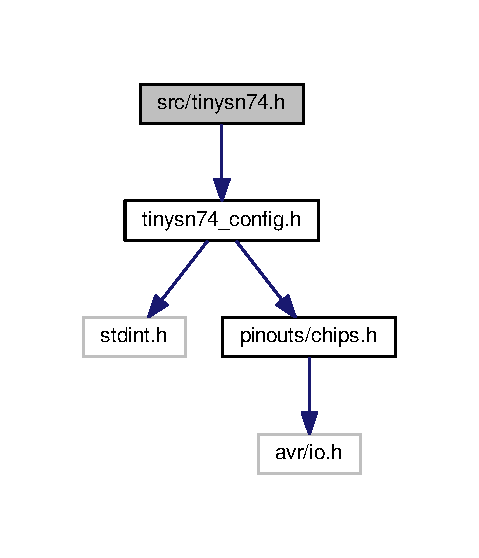
\includegraphics[width=230pt]{tinysn74_8h__incl}
\end{center}
\end{figure}
This graph shows which files directly or indirectly include this file\+:\nopagebreak
\begin{figure}[H]
\begin{center}
\leavevmode
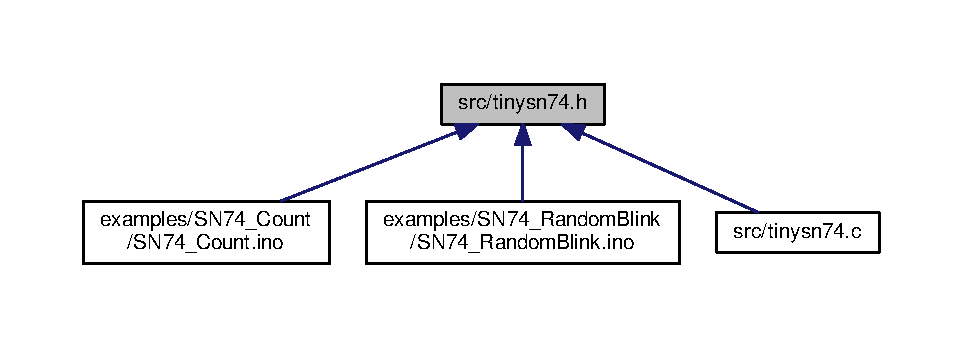
\includegraphics[width=350pt]{tinysn74_8h__dep__incl}
\end{center}
\end{figure}
\subsection*{Functions}
\begin{DoxyCompactItemize}
\item 
void \hyperlink{tinysn74_8h_a75d55e672f3f4dd06cd0c73479f64ade}{sn\+Init} (void)
\begin{DoxyCompactList}\small\item\em Initializes the library. \end{DoxyCompactList}\item 
void \hyperlink{tinysn74_8h_ad06bf9aab33483c64594a58e072279fe}{sn\+C\+LR} (void)
\begin{DoxyCompactList}\small\item\em Clear the output register. \end{DoxyCompactList}\item 
void \hyperlink{tinysn74_8h_ace8f256b6c1b7e959f1d486b8796cb58}{sn\+OE} (uint8\+\_\+t off)
\begin{DoxyCompactList}\small\item\em Enable / disable S\+N74 outputs. \end{DoxyCompactList}\item 
void \hyperlink{tinysn74_8h_ac9f372294bcbd3d976f30953e2aaeb1b}{sn\+Shift\+Init} (void)
\begin{DoxyCompactList}\small\item\em Initializes the shifting logic. \end{DoxyCompactList}\item 
void \hyperlink{tinysn74_8h_aedfd23cb2c8f35f1fd274ad3d9395ad8}{sn\+Shift} (uint8\+\_\+t $\ast$b)
\begin{DoxyCompactList}\small\item\em Shifting logic to get data from the micro to the shift registers. \end{DoxyCompactList}\item 
void \hyperlink{tinysn74_8h_ae57a50787422eaee268c496d51f8dc00}{sn\+Lat} (void)
\begin{DoxyCompactList}\small\item\em Latcn data from S\+N74\textquotesingle{}s internal shift register to the output. \end{DoxyCompactList}\end{DoxyCompactItemize}


\subsection{Function Documentation}
\mbox{\Hypertarget{tinysn74_8h_ad06bf9aab33483c64594a58e072279fe}\label{tinysn74_8h_ad06bf9aab33483c64594a58e072279fe}} 
\index{tinysn74.\+h@{tinysn74.\+h}!sn\+C\+LR@{sn\+C\+LR}}
\index{sn\+C\+LR@{sn\+C\+LR}!tinysn74.\+h@{tinysn74.\+h}}
\subsubsection{\texorpdfstring{sn\+C\+L\+R()}{snCLR()}}
{\footnotesize\ttfamily void sn\+C\+LR (\begin{DoxyParamCaption}\item[{void}]{ }\end{DoxyParamCaption})}



Clear the output register. 

This function will clear all outputs of the connected S\+N74 chips, without having to shift in N bytes of 0x00 \mbox{\Hypertarget{tinysn74_8h_a75d55e672f3f4dd06cd0c73479f64ade}\label{tinysn74_8h_a75d55e672f3f4dd06cd0c73479f64ade}} 
\index{tinysn74.\+h@{tinysn74.\+h}!sn\+Init@{sn\+Init}}
\index{sn\+Init@{sn\+Init}!tinysn74.\+h@{tinysn74.\+h}}
\subsubsection{\texorpdfstring{sn\+Init()}{snInit()}}
{\footnotesize\ttfamily void sn\+Init (\begin{DoxyParamCaption}\item[{void}]{ }\end{DoxyParamCaption})}



Initializes the library. 

This function sets up the ports / pins of the A\+T\+T\+I\+NY to output, and clears the output registers of the connected shift register(s). \mbox{\Hypertarget{tinysn74_8h_ae57a50787422eaee268c496d51f8dc00}\label{tinysn74_8h_ae57a50787422eaee268c496d51f8dc00}} 
\index{tinysn74.\+h@{tinysn74.\+h}!sn\+Lat@{sn\+Lat}}
\index{sn\+Lat@{sn\+Lat}!tinysn74.\+h@{tinysn74.\+h}}
\subsubsection{\texorpdfstring{sn\+Lat()}{snLat()}}
{\footnotesize\ttfamily void sn\+Lat (\begin{DoxyParamCaption}\item[{void}]{ }\end{DoxyParamCaption})}



Latcn data from S\+N74\textquotesingle{}s internal shift register to the output. 

This function is what actually sets the output pins to the value contained in the input shift register. Without calling this, the pins will never go logic high (or logic low). \mbox{\Hypertarget{tinysn74_8h_ace8f256b6c1b7e959f1d486b8796cb58}\label{tinysn74_8h_ace8f256b6c1b7e959f1d486b8796cb58}} 
\index{tinysn74.\+h@{tinysn74.\+h}!sn\+OE@{sn\+OE}}
\index{sn\+OE@{sn\+OE}!tinysn74.\+h@{tinysn74.\+h}}
\subsubsection{\texorpdfstring{sn\+O\+E()}{snOE()}}
{\footnotesize\ttfamily void sn\+OE (\begin{DoxyParamCaption}\item[{uint8\+\_\+t}]{off }\end{DoxyParamCaption})}



Enable / disable S\+N74 outputs. 

If the sn\+OE option is enabled (see tinysn47\+\_\+config.\+h), this function will allow you to enable or disable the output register.

Note that when disabled, the output register retains its previous value -\/ the pins are simply put into high-\/impedance.


\begin{DoxyParams}{Parameters}
{\em off} & uint8\+\_\+t value to pass a \textquotesingle{}0\textquotesingle{} or \textquotesingle{}1\textquotesingle{}. As the chip uses logic low, setting off to \textquotesingle{}0\textquotesingle{} will E\+N\+A\+B\+LE the output register. \\
\hline
\end{DoxyParams}
\mbox{\Hypertarget{tinysn74_8h_aedfd23cb2c8f35f1fd274ad3d9395ad8}\label{tinysn74_8h_aedfd23cb2c8f35f1fd274ad3d9395ad8}} 
\index{tinysn74.\+h@{tinysn74.\+h}!sn\+Shift@{sn\+Shift}}
\index{sn\+Shift@{sn\+Shift}!tinysn74.\+h@{tinysn74.\+h}}
\subsubsection{\texorpdfstring{sn\+Shift()}{snShift()}}
{\footnotesize\ttfamily void sn\+Shift (\begin{DoxyParamCaption}\item[{uint8\+\_\+t $\ast$}]{b }\end{DoxyParamCaption})}



Shifting logic to get data from the micro to the shift registers. 

This function comes in two (2) forms, determined by your selection of D\+A\+T\+A\+\_\+\+X\+F\+E\+R\+\_\+\+M\+OD in \hyperlink{tinysn74__config_8h}{tinysn74\+\_\+config.\+h}.

In bitbang mode (default), the function utilizes a for loop to iterate over the array of chip data. In S\+PI mode, the S\+PI output register and timers are utilized to iterate over the data.


\begin{DoxyParams}{Parameters}
{\em $\ast$b} & is the pointer to the chip array. \\
\hline
\end{DoxyParams}
\mbox{\Hypertarget{tinysn74_8h_ac9f372294bcbd3d976f30953e2aaeb1b}\label{tinysn74_8h_ac9f372294bcbd3d976f30953e2aaeb1b}} 
\index{tinysn74.\+h@{tinysn74.\+h}!sn\+Shift\+Init@{sn\+Shift\+Init}}
\index{sn\+Shift\+Init@{sn\+Shift\+Init}!tinysn74.\+h@{tinysn74.\+h}}
\subsubsection{\texorpdfstring{sn\+Shift\+Init()}{snShiftInit()}}
{\footnotesize\ttfamily void sn\+Shift\+Init (\begin{DoxyParamCaption}\item[{void}]{ }\end{DoxyParamCaption})}



Initializes the shifting logic. 

This function comes in two (2) forms, determined by your selection of D\+A\+T\+A\+\_\+\+X\+F\+E\+R\+\_\+\+M\+OD in \hyperlink{tinysn74__config_8h}{tinysn74\+\_\+config.\+h}.

In bitbang mode (default); the function merely sets pins; whereas in S\+PI mode, the function will also initialize the timers and S\+PI \char`\"{}baudrate\char`\"{}. 
\hypertarget{tinysn74__config_8h}{}\section{src/tinysn74\+\_\+config.h File Reference}
\label{tinysn74__config_8h}\index{src/tinysn74\+\_\+config.\+h@{src/tinysn74\+\_\+config.\+h}}


Master configuration file for the tinysn74 library.  


{\ttfamily \#include $<$stdint.\+h$>$}\newline
{\ttfamily \#include \char`\"{}pinouts/chips.\+h\char`\"{}}\newline
Include dependency graph for tinysn74\+\_\+config.\+h\+:\nopagebreak
\begin{figure}[H]
\begin{center}
\leavevmode
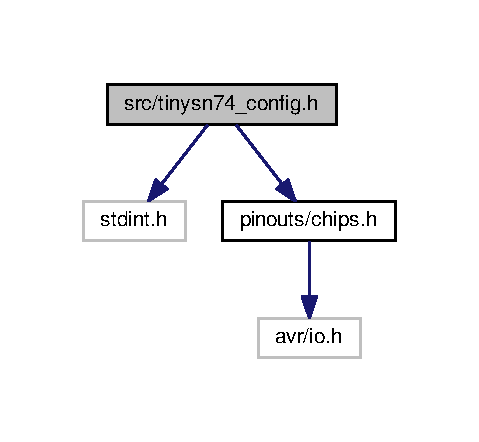
\includegraphics[width=230pt]{tinysn74__config_8h__incl}
\end{center}
\end{figure}
This graph shows which files directly or indirectly include this file\+:\nopagebreak
\begin{figure}[H]
\begin{center}
\leavevmode
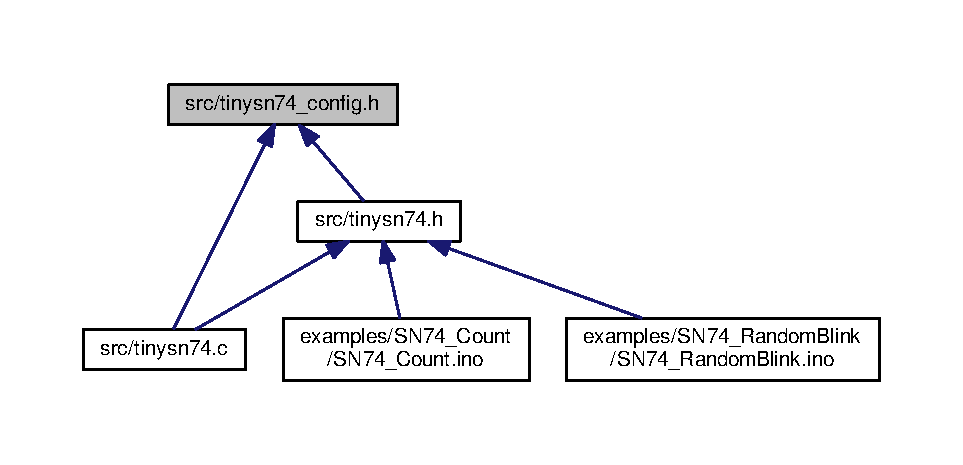
\includegraphics[width=350pt]{tinysn74__config_8h__dep__incl}
\end{center}
\end{figure}
\subsection*{Macros}
\begin{DoxyCompactItemize}
\item 
\mbox{\Hypertarget{tinysn74__config_8h_ac1444f4f02934ebe4ab8e57b71f5b2c6}\label{tinysn74__config_8h_ac1444f4f02934ebe4ab8e57b71f5b2c6}} 
\#define {\bfseries S\+N74\+\_\+\+S\+PI}~1
\item 
\mbox{\Hypertarget{tinysn74__config_8h_a92aeac762162c7b0b526ed6be37e88f1}\label{tinysn74__config_8h_a92aeac762162c7b0b526ed6be37e88f1}} 
\#define {\bfseries S\+N74\+\_\+\+B\+A\+NG}~2
\item 
\mbox{\Hypertarget{tinysn74__config_8h_a80cdfa2921259dcd64bf6a66cd5d0cd2}\label{tinysn74__config_8h_a80cdfa2921259dcd64bf6a66cd5d0cd2}} 
\#define {\bfseries N\+U\+M\+S\+N74}~2
\item 
\mbox{\Hypertarget{tinysn74__config_8h_a73c0947286a79cf4dd7facaa091445dd}\label{tinysn74__config_8h_a73c0947286a79cf4dd7facaa091445dd}} 
\#define {\bfseries S\+N74\+OE}~0
\item 
\mbox{\Hypertarget{tinysn74__config_8h_a8c182bb3254f492c47d29dcff3473954}\label{tinysn74__config_8h_a8c182bb3254f492c47d29dcff3473954}} 
\#define {\bfseries D\+A\+T\+A\+\_\+\+X\+F\+E\+R\+\_\+\+M\+OD}~S\+N74\+\_\+\+B\+A\+NG
\item 
\mbox{\Hypertarget{tinysn74__config_8h_a0101aa3e5dcb00e86ef08075c9eabd19}\label{tinysn74__config_8h_a0101aa3e5dcb00e86ef08075c9eabd19}} 
\#define {\bfseries D\+O\+T\+\_\+\+P\+IN}~D\+E\+F\+\_\+\+M\+O\+S\+I\+\_\+\+P\+IN
\item 
\mbox{\Hypertarget{tinysn74__config_8h_a4f8af5b12a3370a710e09738aec0bf0b}\label{tinysn74__config_8h_a4f8af5b12a3370a710e09738aec0bf0b}} 
\#define {\bfseries D\+O\+T\+\_\+\+P\+O\+RT}~D\+E\+F\+\_\+\+M\+O\+S\+I\+\_\+\+P\+O\+RT
\item 
\mbox{\Hypertarget{tinysn74__config_8h_abc11d7a3aef8551912e35a4f73e5ce61}\label{tinysn74__config_8h_abc11d7a3aef8551912e35a4f73e5ce61}} 
\#define {\bfseries D\+O\+T\+\_\+\+D\+DR}~D\+E\+F\+\_\+\+M\+O\+S\+I\+\_\+\+D\+DR
\item 
\mbox{\Hypertarget{tinysn74__config_8h_a40f496979bb9d7199cca5e0ce136e698}\label{tinysn74__config_8h_a40f496979bb9d7199cca5e0ce136e698}} 
\#define {\bfseries C\+L\+K\+\_\+\+P\+IN}~D\+E\+F\+\_\+\+C\+L\+K\+\_\+\+P\+IN
\item 
\mbox{\Hypertarget{tinysn74__config_8h_a9d3398ed51d28750a7d69fcae8452e25}\label{tinysn74__config_8h_a9d3398ed51d28750a7d69fcae8452e25}} 
\#define {\bfseries C\+L\+K\+\_\+\+P\+O\+RT}~D\+E\+F\+\_\+\+C\+L\+K\+\_\+\+P\+O\+RT
\item 
\mbox{\Hypertarget{tinysn74__config_8h_a52c4d4515980f132b402f7bbe4166287}\label{tinysn74__config_8h_a52c4d4515980f132b402f7bbe4166287}} 
\#define {\bfseries C\+L\+K\+\_\+\+D\+DR}~D\+E\+F\+\_\+\+C\+L\+K\+\_\+\+D\+DR
\item 
\mbox{\Hypertarget{tinysn74__config_8h_a46d935e9a02f4ba391f986bcae4ef83c}\label{tinysn74__config_8h_a46d935e9a02f4ba391f986bcae4ef83c}} 
\#define {\bfseries C\+L\+R\+\_\+\+P\+IN}~D\+E\+F\+\_\+\+C\+L\+R\+\_\+\+P\+IN
\item 
\mbox{\Hypertarget{tinysn74__config_8h_a7d12397cdc36f2235521a535f1088b29}\label{tinysn74__config_8h_a7d12397cdc36f2235521a535f1088b29}} 
\#define {\bfseries C\+L\+R\+\_\+\+P\+O\+RT}~D\+E\+F\+\_\+\+C\+L\+R\+\_\+\+P\+O\+RT
\item 
\mbox{\Hypertarget{tinysn74__config_8h_a051e64c07e3a72f1acda65bd7302176d}\label{tinysn74__config_8h_a051e64c07e3a72f1acda65bd7302176d}} 
\#define {\bfseries C\+L\+R\+\_\+\+D\+DR}~D\+E\+F\+\_\+\+C\+L\+R\+\_\+\+D\+DR
\item 
\mbox{\Hypertarget{tinysn74__config_8h_a2bf8da5ce3f5467e0e72506aa3e85038}\label{tinysn74__config_8h_a2bf8da5ce3f5467e0e72506aa3e85038}} 
\#define {\bfseries L\+A\+T\+\_\+\+P\+IN}~D\+E\+F\+\_\+\+L\+A\+T\+\_\+\+P\+IN
\item 
\mbox{\Hypertarget{tinysn74__config_8h_af6ad52e19906ffe6852754e2f9728781}\label{tinysn74__config_8h_af6ad52e19906ffe6852754e2f9728781}} 
\#define {\bfseries L\+A\+T\+\_\+\+P\+O\+RT}~D\+E\+F\+\_\+\+L\+A\+T\+\_\+\+P\+O\+RT
\item 
\mbox{\Hypertarget{tinysn74__config_8h_ad46055c3cd4d16bdd0cc8c64a12d337d}\label{tinysn74__config_8h_ad46055c3cd4d16bdd0cc8c64a12d337d}} 
\#define {\bfseries L\+A\+T\+\_\+\+D\+DR}~D\+E\+F\+\_\+\+L\+A\+T\+\_\+\+D\+DR
\end{DoxyCompactItemize}


\subsection{Detailed Description}
Master configuration file for the tinysn74 library. 

This file holds the (mostly) static definitions used in the rest of the library. 
%--- End generated contents ---

% Index
\backmatter
\newpage
\phantomsection
\clearemptydoublepage
\addcontentsline{toc}{chapter}{Index}
\printindex

\end{document}
